%%=============================================================================
%% ELK
%%=============================================================================

\chapter{ELK}
\label{ch:ELK}

\section{Installatie en configuratie}
Zoals reeds besproken in Hoofdstuk~\ref{subsec:ELK} ELK, bestaat deze stack uit drie belangrijke elementen die aangevuld kunnen worden met meerdere componenten om deze oplossing efficiënter te maken.
\begin{itemize}
    \item Logstash
    \item Elasticsearch
    \item Kibana
    \item Filebeat (optioneel, vooral in Kubernetes omgevingen)
    \item Message broker zoals Kafka, Redis,... (optioneel, vooral in Kubernetes omgevingen)
\end{itemize}

Logstash is opgebouwd vanuit een pull model. Dit wil zeggen dat Logstash op zoek gaat naar een gedefinieerde input bron waar logs te vinden zijn. Er zijn verschillende inputmogelijkheden zoals file en syslog. Logstash kan ook gebruikt worden met een pushmodel. Het stelt zichzelf open om logs te ontvangen van Filebeats om deze verder te verwerken en door te sturen naar Elasticsearch. Om deze demonstratie eenvoudig voor te stellen wordt gebruik gemaakt van een log generator plugin van Elastic. Deze plugin configuratie is te zien in Listing 4.1. Zo kan gefocust worden op de drie belangrijkste componenten.

\subsection{Lokale omgeving}

De eenvoudigste manier om een snelle testomgeving op te stellen is door gebruik te maken van een github repositoy met reeds bestaande configuratie en deze naar eigen wens aan te passen. Met de repository https://github.com/deviantony/docker-elk kan mits enkele aanpassingen een ELK stack uitgerold worden. Hierbij moet de input van de Logstash config in de pipeline folder nog aangepast worden naar de log generator die te zien is in Listing 4.1. Verder wordt gebruik gemaakt van een docker-compose.yaml file om alle services met één commando uit te rollen. Door het gebruik van authenticatie bij deze installatie moet ingelogd worden bij Kibana om verder te gaan. De inloggegevens zijn ook te vinden in de repository. 

Eens de setup uitgerold is moet er een index gecreëerd worden in Kibana om de logs te kunnen filteren. Daarna zijn de logs te zien in de `Discover` pagina zoals te zien is in Figure 4.1.


\begin{lstlisting}[caption=Log generator plugin config Logstash]
input {
    generator {
        lines => [
            "Dit is een test log",
            "Tweede test log",
            "Nog een test log"
        ]
        # Emit all lines 25 times.
        count => 25
    }
}
\end{lstlisting}

\begin{figure}[ht]
    \centering
    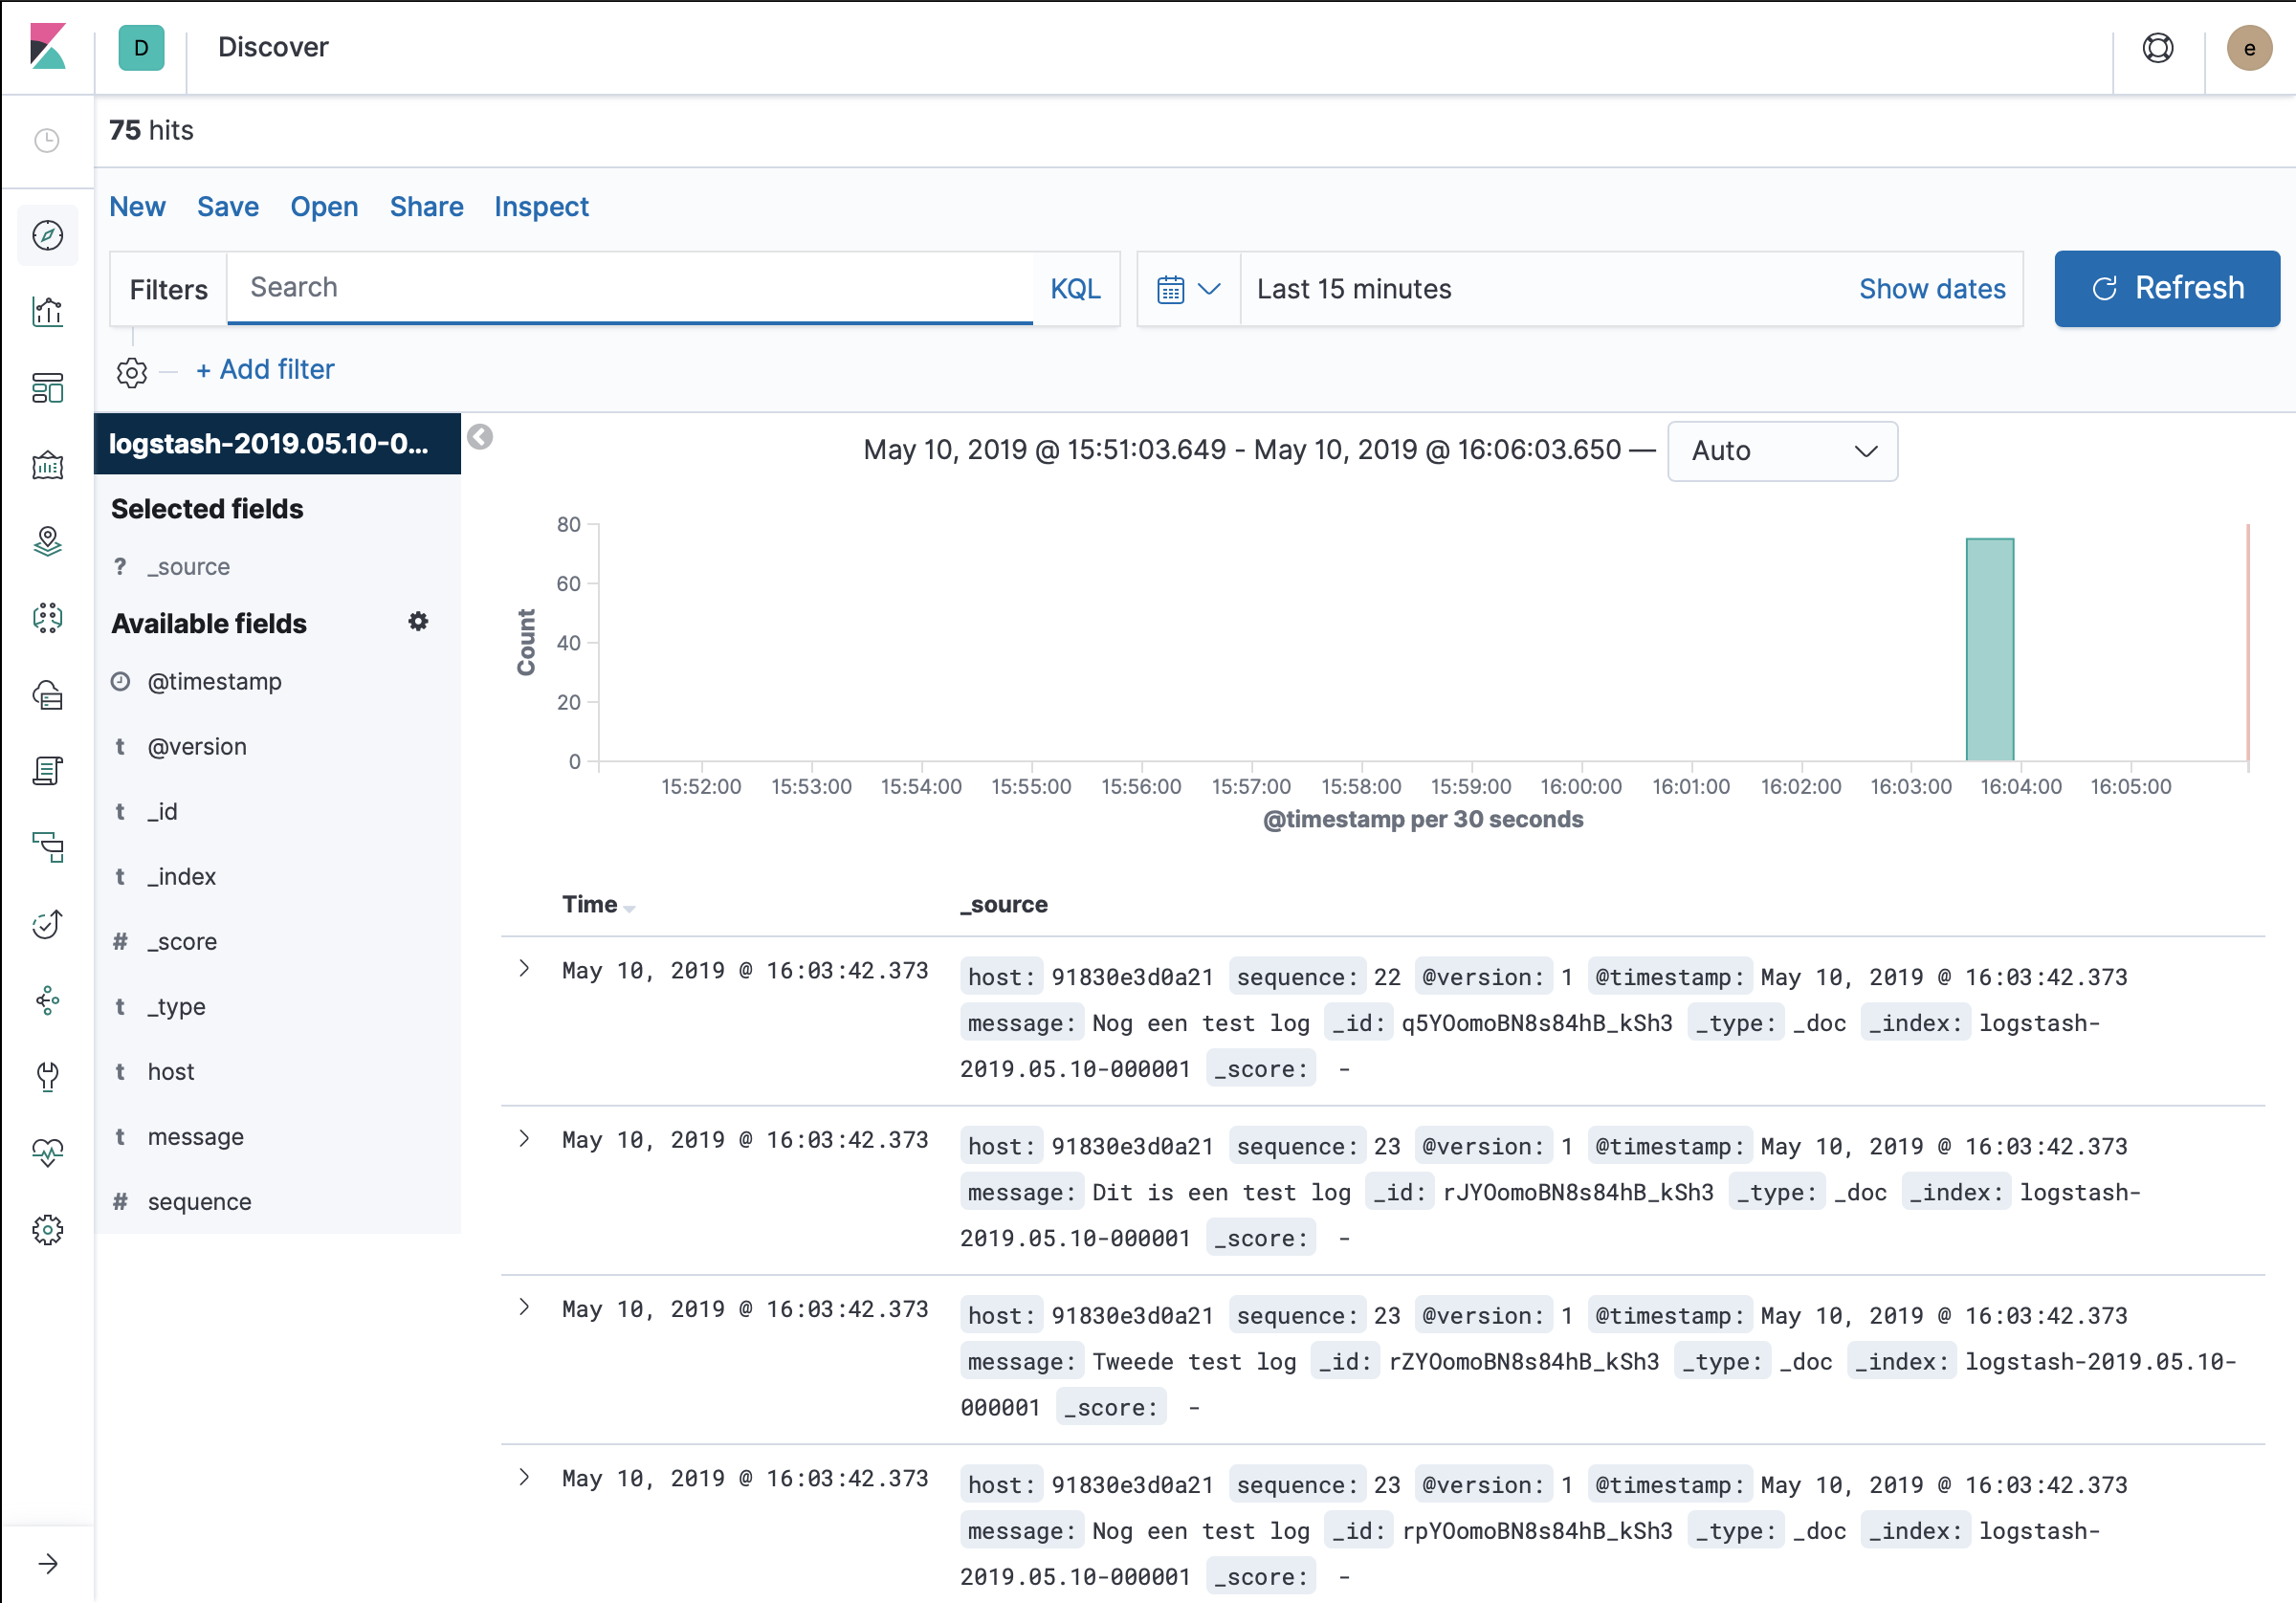
\includegraphics[scale=0.35]{img/ELK-stack-frontend}
    \caption[ELK stack frontend]{ELK stack frontend}
\end{figure}

\subsection{Kubernetes omgeving}

De configuratie van de ELK stack voor Kubernetes is ingewikkelder. Hierbij wordt gebruik gemaakt van een StatefulSet voor de configuratie van Elasticsearch. Dit is lijkt op een gewone Deployment maar heeft enkele verschillen. De belangrijkste is dat elke replica van een Deployment exact hetzelfde is en deze dus uitwisselbaar zijn. In tegenstelling tot alle replicas van een StatefulSet. Deze zijn gebaseerd op eenzelfde configuratie maar zijn niet uitwisselbaar vanwege een unieke, gepersisteerde identifier. StatefulSets worden gebruikt stabiele networken opgebouwd moeten worden met een persistent storage.

De volledige configuratie is buiten de scope van dit onderzoek en zal dus niet besproken worden. De documentatie van Elastic biedt veel ondersteuning bij het opzetten van een eigen Elastic stack.

\section{Requirements}

\subsection{Must have}
\subsubsection{Moet open source zijn}
Voor elk van de onderzochte oplossingen geldt dezelfde score voor deze requirement, namelijk 5. Elk van de componenten waaruit een ELK of Elastic stack bestaat is vrij te verkrijgen en te gebruiken.

\subsubsection{Ondersteuning voor cluster omgevingen zoals Kubernetes}
In de documentatie van Elastic \autocite{elastic} zijn er verschillende links te vinden die een stap voor stap begeleiding geven om deze stack werkende te krijgen. Er zijn ook videos dit nogmaals aantonen dat er een goede ondersteuning is voor Kubernetes.

Om deze redenen zal hiervoor een 4 gegeven voor deze requirement.

\subsubsection{Moet een zo klein mogelijke impact hebben op de servers}
Bij velen is het al geweten dat Elasticsearch een grote impact heeft op het systeem waar het geïmplementeerd is. Een eerste argument hiervoor is de JVM (Java Virtual Machine) waarmee Elasticearch werkt. Deze heeft volgens \cite{elasticheap} een standard minimum heap size van 1GB maar wordt in productie snel omhoog gescaled om ervoor te zorgen dat Elasticsearch functioneel blijft. Dit in combinatie met de best practice voor het installeren op Kubernetes gebruikt door \cite{swidler2018} waarin minstens 3 nodes van Elasticsearch aangemaakt worden, zorgt meteen al voor een hoog RAM gebruik. Een tweede argument hiervoor is de manier waarop Elasticsearch data, in de geval logs, opslaat. Dit gebeurt door middel van volledige indexering waardoor de benodigde opslagruimte groter zal zijn dan andere databanken die indexering vermijden of slecht enkele delen van de data indexeren. 

De combinatie van deze twee argumenten zorgt voor een relatief grote impact op de servers. Daarom krijgt de ELK of Elastic stack een score van 2 voor dit requirement.

\subsubsection{Moet kunnen scalen naargelang de groeiende Kubernetes cluster}
Indien gebruik gemaakt wordt van een DaemonSet voor de configuratie van FileBeats zal het aantal FileBeat containers automatisch gescaled worden bij het aanmaken van nieuwe pods. Wanneer de Kubernetes cluster een bepaalde grootte heeft, zal ook het aantal Elasticsearch nodes groeien. Deze kunnen automatisch gescaled worden met de correcte configuratie.

Indien gesteld wordt dat de oorspronkelijke configuratie correct is gebeurd, kan gesteld worden dat de ELK of Elastic stack automatisch scaled naargelang de groei van de cluster. Daarom krijgt de ELK of Elastic stack een score van 5 voor deze requirement.

\subsection{Should have}
\subsubsection{Moet (relatief) eenvoudig te configureren zijn}
De best practices om Elasticsearch te configureren op Kubernetes zijn dat er minsten 3 nodes aangemaakt moeten worden. 1 master en meerdere data nodes. Er zijn talloze manieren waarop Elasticsearch kan geïnstalleerd worden en heel wat zaken die kunnen mislopen.

FileBeat, Logstash, en Kibana zijn eenvoudig te configureren en vormen geen probleem, zowel lokaal als op Kubernetes. 

Om deze redenen krijgt de ELK of Elastic stack een 2 voor dit requirement

\subsubsection{Moet (relatief) eenvoudig te gebruiken zijn}
De leercurve om gebruik te maken van Elasticsearch is vrij hoog, terwijl de leercurve om gebruik te maken van Kibana relatief laag is.

Voor de requirement krijgt de ELK of Elastic stack een score van 4.

\subsubsection{Moet goed gedocumenteerd zijn}
Dankzij de maturiteit van Elastic is er reeds veel documentatie aanwezig, zowel in de vorm van eigen documentatie en documentatie vanuit de user community. De documentatie van Elastic zelf is zeer uitgebreid voor algemeen gebruik maar voor speciale use cases zal vaak eerder documentatie van de community gebruikt moeten worden.

Voor de requirement krijgt de ELK of Elastic stack een score van 4.

\subsubsection{Moet de logs overzichtelijk kunnen tonen}
De frontend van ELK of Elastic stack is Kibana. Deze zorgt voor een overzichtelijke visualisatie van alle logs. Dankzij de volledige indexering van de data binnen Elasticsearch, is er een uitgebreid filtersysteem waar Kibana gebruik van kan maken. Ook kunnen er deep text queries uitgevoerd worden.

Om deze redenen krijgt de ELK of Elastic stack een 5 voor deze requirement.

\subsubsection{Ondersteuning voor verschillende plugins die data extra kunnen verwerken of naar meerdere locaties kunnen doorsturen}
Filebeat is de logcollector die de logs doorstuurt naar Logstash. Logstash zelf heeft een aantal ondersteunde plugins die gebruikt kunnen worden. Zo kan het een groot aantal inputs verwerken en de data doorsturen naar een groot aantal outputs. Dataverwerking plugins zijn ook beschikbaar maar in mindere mate.

Om deze redenen krijgt de ELK of Elastic stack een 3 voor deze requirement

\subsubsection{Ondersteuning voor visualisatie zoals grafieken}
Kibana voorziet functionaliteit voor het produceren van grafieken. Verschillende soorten grafieken en tellers zijn ondersteund.

Voor de requirement krijgt de ELK of Elastic stack een score van 5.

\subsection{Could have}
\subsubsection{Ondersteuning voor alerts}
Kibana voorziet functionaliteit voor alerts. Deze alerts kunnen via verschillende kanalen verzonden worden. 

Voor de requirement krijgt de ELK of Elastic stack een score van 5.

\section{Resultaten}
Zoals te zien is in tabel~\ref{tab:ELK-resultaten} scoort de ELK stack een 2 op een Must Have requirement, namelijk `Moet een zo klein mogelijke impact hebben op de servers`. Dit wijst erop dat ELK niet geschikt is voor grote clusters. Hoe groter de cluster, hoe groter de impact. Het scoort goed op overzichtelijkheid en functionaliteit. 

Een uitgebreide conclusie is te vinden in Hoofdstuk~\ref{ch:conclusie} Conclusie.

\begin{table}[ht]
    \begin{tabular}{| m{20em} | m{2cm} | m{2cm} | m{2cm} |}
        \hline
        \textbf{Requirement}                                                                                              & \textbf{Score (op 5)} & \textbf{Multiplier} & \textbf{Score met multiplier} \\ \hline
        Moet open source zijn                                                                                             & 5                     & 10                  & 50                            \\ \hline
        Ondersteuning voor cluster omgevingen zoals Kubernetes                                                            & 4                     & 10                  & 40                            \\ \hline
        Moet een zo klein mogelijke impact hebben op de servers                                                           & 2                     & 10                  & 20                            \\ \hline
        Moet kunnen scalen naargelang de groeiende Kubernetes cluster                                                     & 5                     & 10                  & 50                            \\ \hline
        Moet (relatief) eenvoudig te configureren zijn                                                                    & 2                     & 5                   & 10                            \\ \hline
        Moet (relatief) eenvoudig te gebruiken zijn                                                                       & 4                     & 5                   & 20                            \\ \hline
        Moet goed gedocumenteerd zijn                                                                                     & 4                     & 5                   & 20                            \\ \hline
        Moet de logs overzichtelijk kunnen tonen                                                                          & 5                     & 5                   & 25                            \\ \hline
        Ondersteuning voor verschillende plugins die data extra kunnen verwerken of naar meerdere locaties kan doorsturen & 3                     & 5                   & 15                            \\ \hline
        Ondersteuning voor visualisatie zoals grafieken                                                                   & 5                     & 5                   & 25                            \\ \hline
        Ondersteuning voor alerts                                                                                         & 5                     & 1                   & 5                             \\ \hline
        \textbf{Totale score}                                                                                             & 39                    &                     & 280                           \\ \hline
    \end{tabular}
    \caption{ELK resultaten}
    \label{tab:ELK-resultaten}
\end{table}


